\section{Metodologia de Desenvolvimento}

Para se construir um software é necessário seguir uma série de passos previsíveis, esses passos estão definidos no processo de software. De acordo com \cite{pressman} um processo de software pode ser visto como um conjunto de atividades, métodos, práticas e transformações que guiam pessoas na produção de software.

Para a construção do processo há uma adaptação em 3 principais níveis de acordo com o \cite{safe} (portfólio, programa e time):

\begin{itemize}
  \item O nível de portfólio será utilizado para gerar boa parte da documentação do projeto aplicando as 3 atividades principais da engenharia de requisitos, que são elicitação, modelagem e análise;
  \item O nível de programa tem como artefatos o documento de arquitetura, as ferramentas de UX e o product backlog com sua rastreabilidade;
  \item O nível de time que é onde codificar a solução, está dividido em desenvolvimento que irá executar a sprint e gestão na qual irá aplicar as práticas do scrum, além da infraestrutura e dos testes.
\end{itemize}

A construção do software será feito seguindo uma adaptação das metodologias ágeis SCRUM, XP e SAFe para aumentar a produtividade e eficiência do mesmo, já que o projeto todo será feito por uma única pessoa, ou seja, terá toda uma adaptação para isso.

Foi decidido o SCRUM devido a grande familiaridade que o desenvolvedor tem com a metodologia, ela é bastante utilizada no mercado e muito útil para organização, controle e gerenciamento do projeto. O XP também já é bem utilizado e conhecido por ser uma metodologia de desenvolvimento de software que ajuda a criar sistemas de melhor qualidade e o SAFe, este é bastante útil para padronizar o processo de forma organizada.

Nesse projeto, para criar o processo de desenvolvimento, foi realizado algumas adaptações a essas metodologias:

\begin{itemize}
  \item \textbf{Papeis}: As metodologias citadas apresentam alguns papéis que devem ser focados pela equipe, porém como o projeto será todo realizado por um único membro os papéis não se tornam relevantes ao projeto.
  \item \textbf{SCRUM}: O SCRUM tem alguns rituais como o daily que para um único membro não se torna necessária.
  \item \textbf{XP}: Uma das práticas citadas do XP que não será utilizada é a programação pareada.
  \item \textbf{SAFe}: Do SAFe será aproveitado somente os padrões de organização do processo em níveis e a rastreabilidade dos requisitos.
\end{itemize}

\subsection{Processo de Engenharia de Requisitos: Nível de Portfólio}

Dentro da Engenharia de Software vários modelos definem as etapas necessárias para se construir um software de acordo
com o processo definido, mas todos têm algo em comum: uma etapa dedicada a compreensão dos problemas a serem
solucionados e a definição do quê será feito. Esta etapa inicial recebe o nome de engenharia de requisitos e está
localizado no nível de portfólio do SAFe.

O processo definido na figura \ref{fig:requisitos} para a etapa de engenharia de requisitos do software PGTBL segue três fases principais:

\begin{itemize}
  \item \textbf{Elicitação}: Essa atividade preocupa-se com o levantamento dos principais aspectos, sejam eles funcionais e/ou não funcionais. Podemos dizer que passamos de um alto nível de abstração para algo mais próximo do mundo real utilizando várias técnicas de elicitação, no caso foi utilizado as técnicas de brainstorm e prototipagem.
  \item \textbf{Modelagem}: Uma vez elicitados os requisitos, deve-se modelar os mesmo de acordo com uma notação adequada, foi utilizado o framework i* para uma modelagem mais organizacional do projeto, o UML para requisitos funcionais do projeto através do diagrama de classe e o framework NFR para requisitos não funcionais do projeto.
  \item \textbf{Análise}: Essa atividade usa a modelagem para obter maior conhecimento sobre as necessidades do software em investigação, no caso os planos de análise de riscos, custos, tempo, viabilidade técnica e outros aspectos são levados em consideração.
\end{itemize}

\begin{figure}[h!]
	\centering
  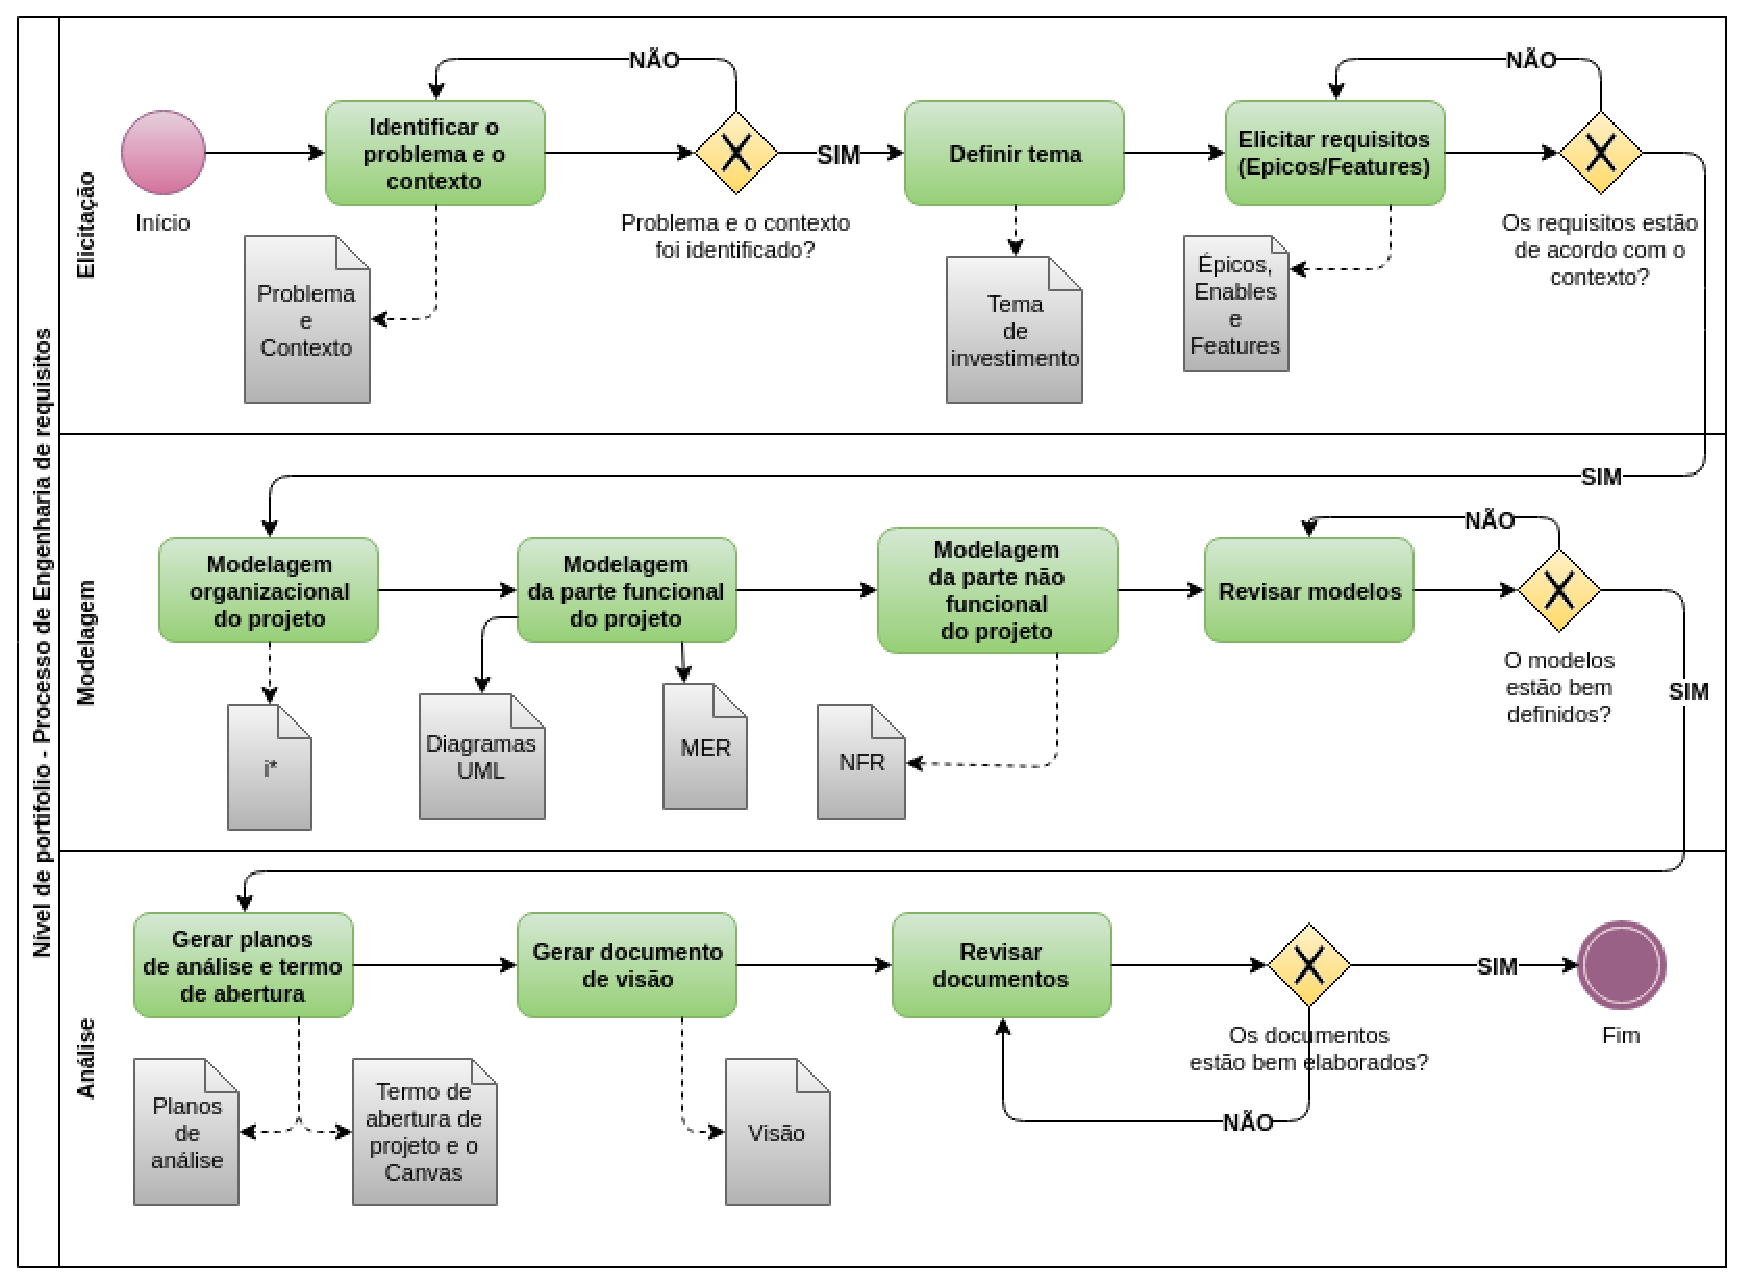
\includegraphics[keepaspectratio=true,scale=0.5]{figuras/requisitos.eps}
  \caption[Processo de engenharia de requisitos.]{Processo de engenharia de requisitos. Fonte: Autor}
	\label{fig:requisitos}
\end{figure}

\subsubsection{Elicitação}

Em paralelo ao processo do TCC o processo de desenvolvimento se inicia com o subprocesso de engenharia de requisitos na parte de elicitação. Esse tem como pontapé inicial identificar o problema e o contexto na qual o software será aplicado e definir o tema de investimento. É nessa fase que é identificado os épicos (requisitos funcionais) e enables (requisitos não funcionais) através de técnicas de elicitação como brainstorms e prototipação. Com isso os épicos (EP) são separados em pedaços menores chamados Features (EN).

\subsubsection{Modelagem}

Na fase de modelagem objetiva-se criar um modelo organizacional em contexto com o uso do software, diagramas que auxilia na construção das funcionalidades por meio da modelagem UML, por exemplo, diagrama de classe, além de criar a modelagem do banco de dados relacional utilizando a modelo entidade relacionamento (MER). Na parte não funcional será criado diagramas que auxilia a identificação e rastreabilidade de requisitos não funcionais como metas a serem alcançadas através do framework NFR.

\subsubsection{Análise}

Na fase de análise objetiva-se criar todos os documentos relacionados ao gerenciamento do projeto, por exemplo, documento de abertura de projeto, plano de gerenciamento de recursos humanos, comunicação, risco, medição e análise, configuração de software, aquisição e custos. Além disso nessa fase será elaborado o documento de visão do projeto.
